% =======================================================================================
% =======================================================================================
% === IMPORTANT NOTE FOR STUDENTS:                                                    ===
% =======================================================================================
% === Do NOT change anything in this file. Only change files in the "reportContent"   ===
% === subfolder.                                                                      ===
% =======================================================================================
% =======================================================================================

\documentclass[runningheads,a4paper]{llncs}
\usepackage{makeidx}
%\usepackage{chapterbib}
\usepackage[ngerman,english]{babel}
\selectlanguage{english}

\usepackage[utf8]{inputenc}
\usepackage[T1]{fontenc}

\usepackage{csquotes}
\usepackage{xpatch} % Recommended for biblatex
\usepackage[backend=biber,style=numeric,language=english]{biblatex} % pdflatex -> biber -> pdflatex (2x)


\usepackage{graphicx}


 
\usepackage{import}
\usepackage{lipsum}
\usepackage{setspace}
\usepackage{pdfpages}


% =======================================================================================
% === The following latex-packages should cover all your needs.                       ===
% === If this is not the case, please write an email to one of the assistants in      ===
% === which you inform us which additional package you need and why.                  ===
% === (Otherwise we will not be able to generate proceedings for the course...)       ===
% =======================================================================================

% For curly underline
\usepackage[normalem]{ulem}

% For URLs
\usepackage{xurl}
\usepackage[hidelinks]{hyperref}

% For Subfigures
\usepackage{subfig}

% For Algorithms
\usepackage{algorithmic}
\usepackage{algorithm}

% For Code Snippets
\usepackage{listings}

% For Todo Notes 
\usepackage[colorinlistoftodos]{todonotes}

% For Colors (\textcolor etc.)
\usepackage{color}

% For Tables
\usepackage{multirow}

% For Tikz
\usepackage{tikz}

% For References
\usepackage{cleveref}

% Required for turning proceedings on and off
% (Source: http://tex.stackexchange.com/questions/87656/turning-parts-of-text-on-and-off)
\usepackage{etoolbox}
\usepackage{verbatim}

\newbool{produceProceedings}
\newbool{produceProceedingsBookVersion}
\newenvironment{produceProceedings}{}{}


%
%
% procedureProceedings : boolean
% ==============================
%
% If true: Generates the proceedings - Only compile with proceedings.py then
% If false: Generates the plain article (typically student mode).
%
% _______________________
% Note for the assistants: Change to true in order to generate the proceedings.
%                          DO NOT compile this file directly when set to true.
%
\setbool{produceProceedings}{false}


\ifbool{produceProceedings}{


%
%
% produceProceedingsBookVersion : boolean
% =======================================
%
% If true: Inserts empty pages so that every report start on an odd page which helps to print the proceedings as double pages.
% If false: No empy pages are inserted.
%
% _______________________
% Note for the assistants: Change to true in order to generate the proceedings which adds empty pages to start every report on an odd page.
%
\setbool{produceProceedingsBookVersion}{false}



}{\AtBeginEnvironment{produceProceedings}{\comment}\AtEndEnvironment{produceProceedings}{\endcomment}}


%
%
% coursename : String
% ===================
%
% Name of the course / lecture.
%
\newcommand{\coursename}{Databases lecture}


%
%
% courseacronym : String
% ======================
%
% Acronym of the course (e.g., DIS for Distributed Information Systems, or CS244 for Databases).
%
\newcommand{\courseacronym}{cs244}


%
%
% semester : String
% =================
%
% The semester (e.g., spring semester 2018 or autumn semester 2018).
%
\newcommand{\semester}{autumn semester 2019}


%
%
% Semester : String
% =========================
%
% The semester with startring capital letters.
%
\newcommand{\Semester}{Autumn Semester 2019}


%
%
% proceedingsSubtitle : String
% ============================
%
% Subtitle of the proceedings.
%
\newcommand{\proceedingsSubtitle}{Project Reports}

%
%
% lectureInstitute : String
% ============================
%
% Combination of lecture and institute information
%
\newcommand{\lectureInstitute}{University of Basel \\ \coursename\ (\courseacronym) \\ \Semester}

%
%
% report : Environment
% ============================
%
% Environment to put the report in.
% Prepends the title and Appends the (local) bilbiography
%
\newenvironment{report}
    {
        \ifbool{produceProceedingsBookVersion}{\cleardoublepage}{}
        \begin{refsection}
            \maketitle
    }
    {
            \printbibliography
        \end{refsection}
    }


%
%
% rootDocument : String
% =====================
%
% Set the to this document's file name.
%
\newcommand{\rootDocument}{proceedings.tex}
\newcommand{\rootName}{proceedings}


\ifbool{produceProceedings}
{
    % Proceedings - Create the entire proceedings in all its glory.
    \input{bibliography.tex}
    \input{graphics.tex}
}{
    % No proceedings - single report. Usually only used by a student group during writing.
    \addbibresource{./reportContent/report.bib}
    \graphicspath{{images/}{reportContent/images/}}
}



\begin{document}
	
\begin{produceProceedings}
	
	\begin{titlepage}
		
\includegraphics{UniBas_Logo_EN_Schwarz_RGB_65}
		
		\vspace{80pt}
		
		\centering
		
		\begin{spacing}{2.8}
		{\Huge \fontfamily{phv} \bfseries Proceedings of the \coursename\ (\courseacronym)}
		\end{spacing}
		
		\vspace{25pt}
		
		{\large \proceedingsSubtitle}
		
		\vspace{50pt}
		
		{\large \Semester}
		
		\vspace{50pt}
		
		{\large	Department of Mathematics and Computer Science}
		
		\vspace{5pt}
		
		{\large Faculty of Science}
		
		\vspace{25pt}
		
		{\large	University of Basel}
	\end{titlepage}
	
	\ifbool{produceProceedingsBookVersion}{\frontmatter}{}
	
	\pagestyle{headings}
	\addtocmark{Reports}
	%
	\chapter*{Preface}
	This documents contains all student reports of the \coursename\ (\courseacronym) held at the University of Basel in the \semester.
	%
	\chapter*{Organization}
	The \coursename\ (\courseacronym) of the \semester\ is organized by the Databases and Information Systems (DBIS) research group, Department of Mathematics and Computer Science, University of Basel.
	%
	\section*{Lecturer}
	Prof.\,Dr. Heiko Schuldt (heiko.schuldt@unibas.ch)
	%
	\section*{Assistants}
	Sein Coray, MSc. (s.coray@unibas.ch)\\
	Silvan Heller, MSc. (silvan.heller@unibas.ch)\\
	Loris Sauter, MSc. (loris.sauter@unibas.ch)\\
	Alexander Stiemer, MSc. (alexander.stiemer@unibas.ch)
	%
%	\section*{Tutors}
    %% Add Tutors (Teaching Assistants) as needed
	%
	\tableofcontents
\end{produceProceedings}
	
%
\mainmatter
%


\ifbool{produceProceedings}{
    \documentclass[12pt]{article}

% -- Packages --
\usepackage{graphicx}
\graphicspath{{images/}}
\usepackage{fancyhdr}
\usepackage{vmargin}
\usepackage{subfig}
\usepackage{lipsum}
\usepackage{color}
% --

% NO TOUCHY
%------------------------------------------------------------------
\setmarginsrb{3 cm}{2.5 cm}{3 cm}{2.5 cm}{1 cm}{1.5 cm}{1 cm}{1.5 cm}
\pagestyle{fancy}
\fancyhf{}
\cfoot{\thepage}
%------------------------------------------------------------------


\begin{document}

% -- TITLE PAGE --
\begin{titlepage}
	\centering
    \vspace*{0.5 cm}
    
\includegraphics[scale = 0.5]{images/unibas_logo.jpeg}\\[1.0 cm]
    \textsc{\LARGE  The 2016 US elections and suicide rates in the US}\\[2.0 cm]
    \textsc{ COMPUTER SCIENCE DEPARTMENT}\\[0.2 cm]
	\textsc{DATABASES - \textbf{P3}: Analysis and visualisation}\\[0.2cm]
	\textsc{\Large FS 2019}\\[0.5 cm]
	\rule{\linewidth}{0.2 mm} \\[0.4 cm]

	\begin{minipage}{0.4\textwidth}

			\begin{flushright}
			\emph{STUDENT IDS :} \\
				Rik De Graaf {\color{red}12345678}\linebreak
			Travis Rivera Petit 15-117-427\linebreak
		\end{flushright}
	\end{minipage}\\[2 cm]


	\vfill

\end{titlepage}
% --

%\tableofcontents
%\pagebreak


\section{INTRODUCTION}
{\color{red}problem}\\
"To what extent have the result of the US 2016 presidential
elections affected the suicide rates in the United States?"

{\color{red} analysis goals}\\
The rise of social media has given people from all different
backgrounds a plattform with which to share their thoughts
and feelings online leaving them avaiable for anyone to read.
This phenomenon gives society yet another tool for analysing
people's mass behavior; after all, if many individuals share
similar posts online, it may be a sign that something
is going on.
This becomes particualrly interesting
when important events that affect everyone in a contry take
palce.

After the last US elections,
some were hearly displeased and others
satisfied, this friction has been pronounced by the fact
that the controvesial figure Donald Trump has taken over
the presiency of the United States since 2016.

Many opposers of Trump did not stop at Twitter or Reddit, they
took it up to themselves to go out and protest on the streets.

Our aim is to use information about protests, riots, and
related events together with the results of the elections
and the suicide rates to make a conty-level investigation
regarding the question above.



%{\color{red} sources}\\


\section{SOURCE MATERIAL}
everything about our data sets and how we go about modeleing it.
The ER diagrams and such belong here.


\section{INTEGRATION}
The GDELT data subset we use in this project consists of sixty
three thousand csv files, where each file takes somewhere between
800 KB and 1.5 MB of storage.

On our P2 hand-in we include a script
(/gdelt/download.py) that downloads each csv file
and edits the filenames for further processing.
If a file is found to be corrupt, it is not downloaded and
the index of the file is saved in a .txt file
(/gdelt/bad\_indices.txt).

The dataset consists of sixty attributes and the domain of
each attribute is in detail on the official handbook
{\color{red}{citation}}.

Moving on, the suicide rate dataset can be obtained from
the Centers for Disease Control and Prevention
website \cite{suicide_website}.

The election results dataset is straightforward, it can be
obtained on {\color{red}{todo}}.

\begin{figure}
	\centering
	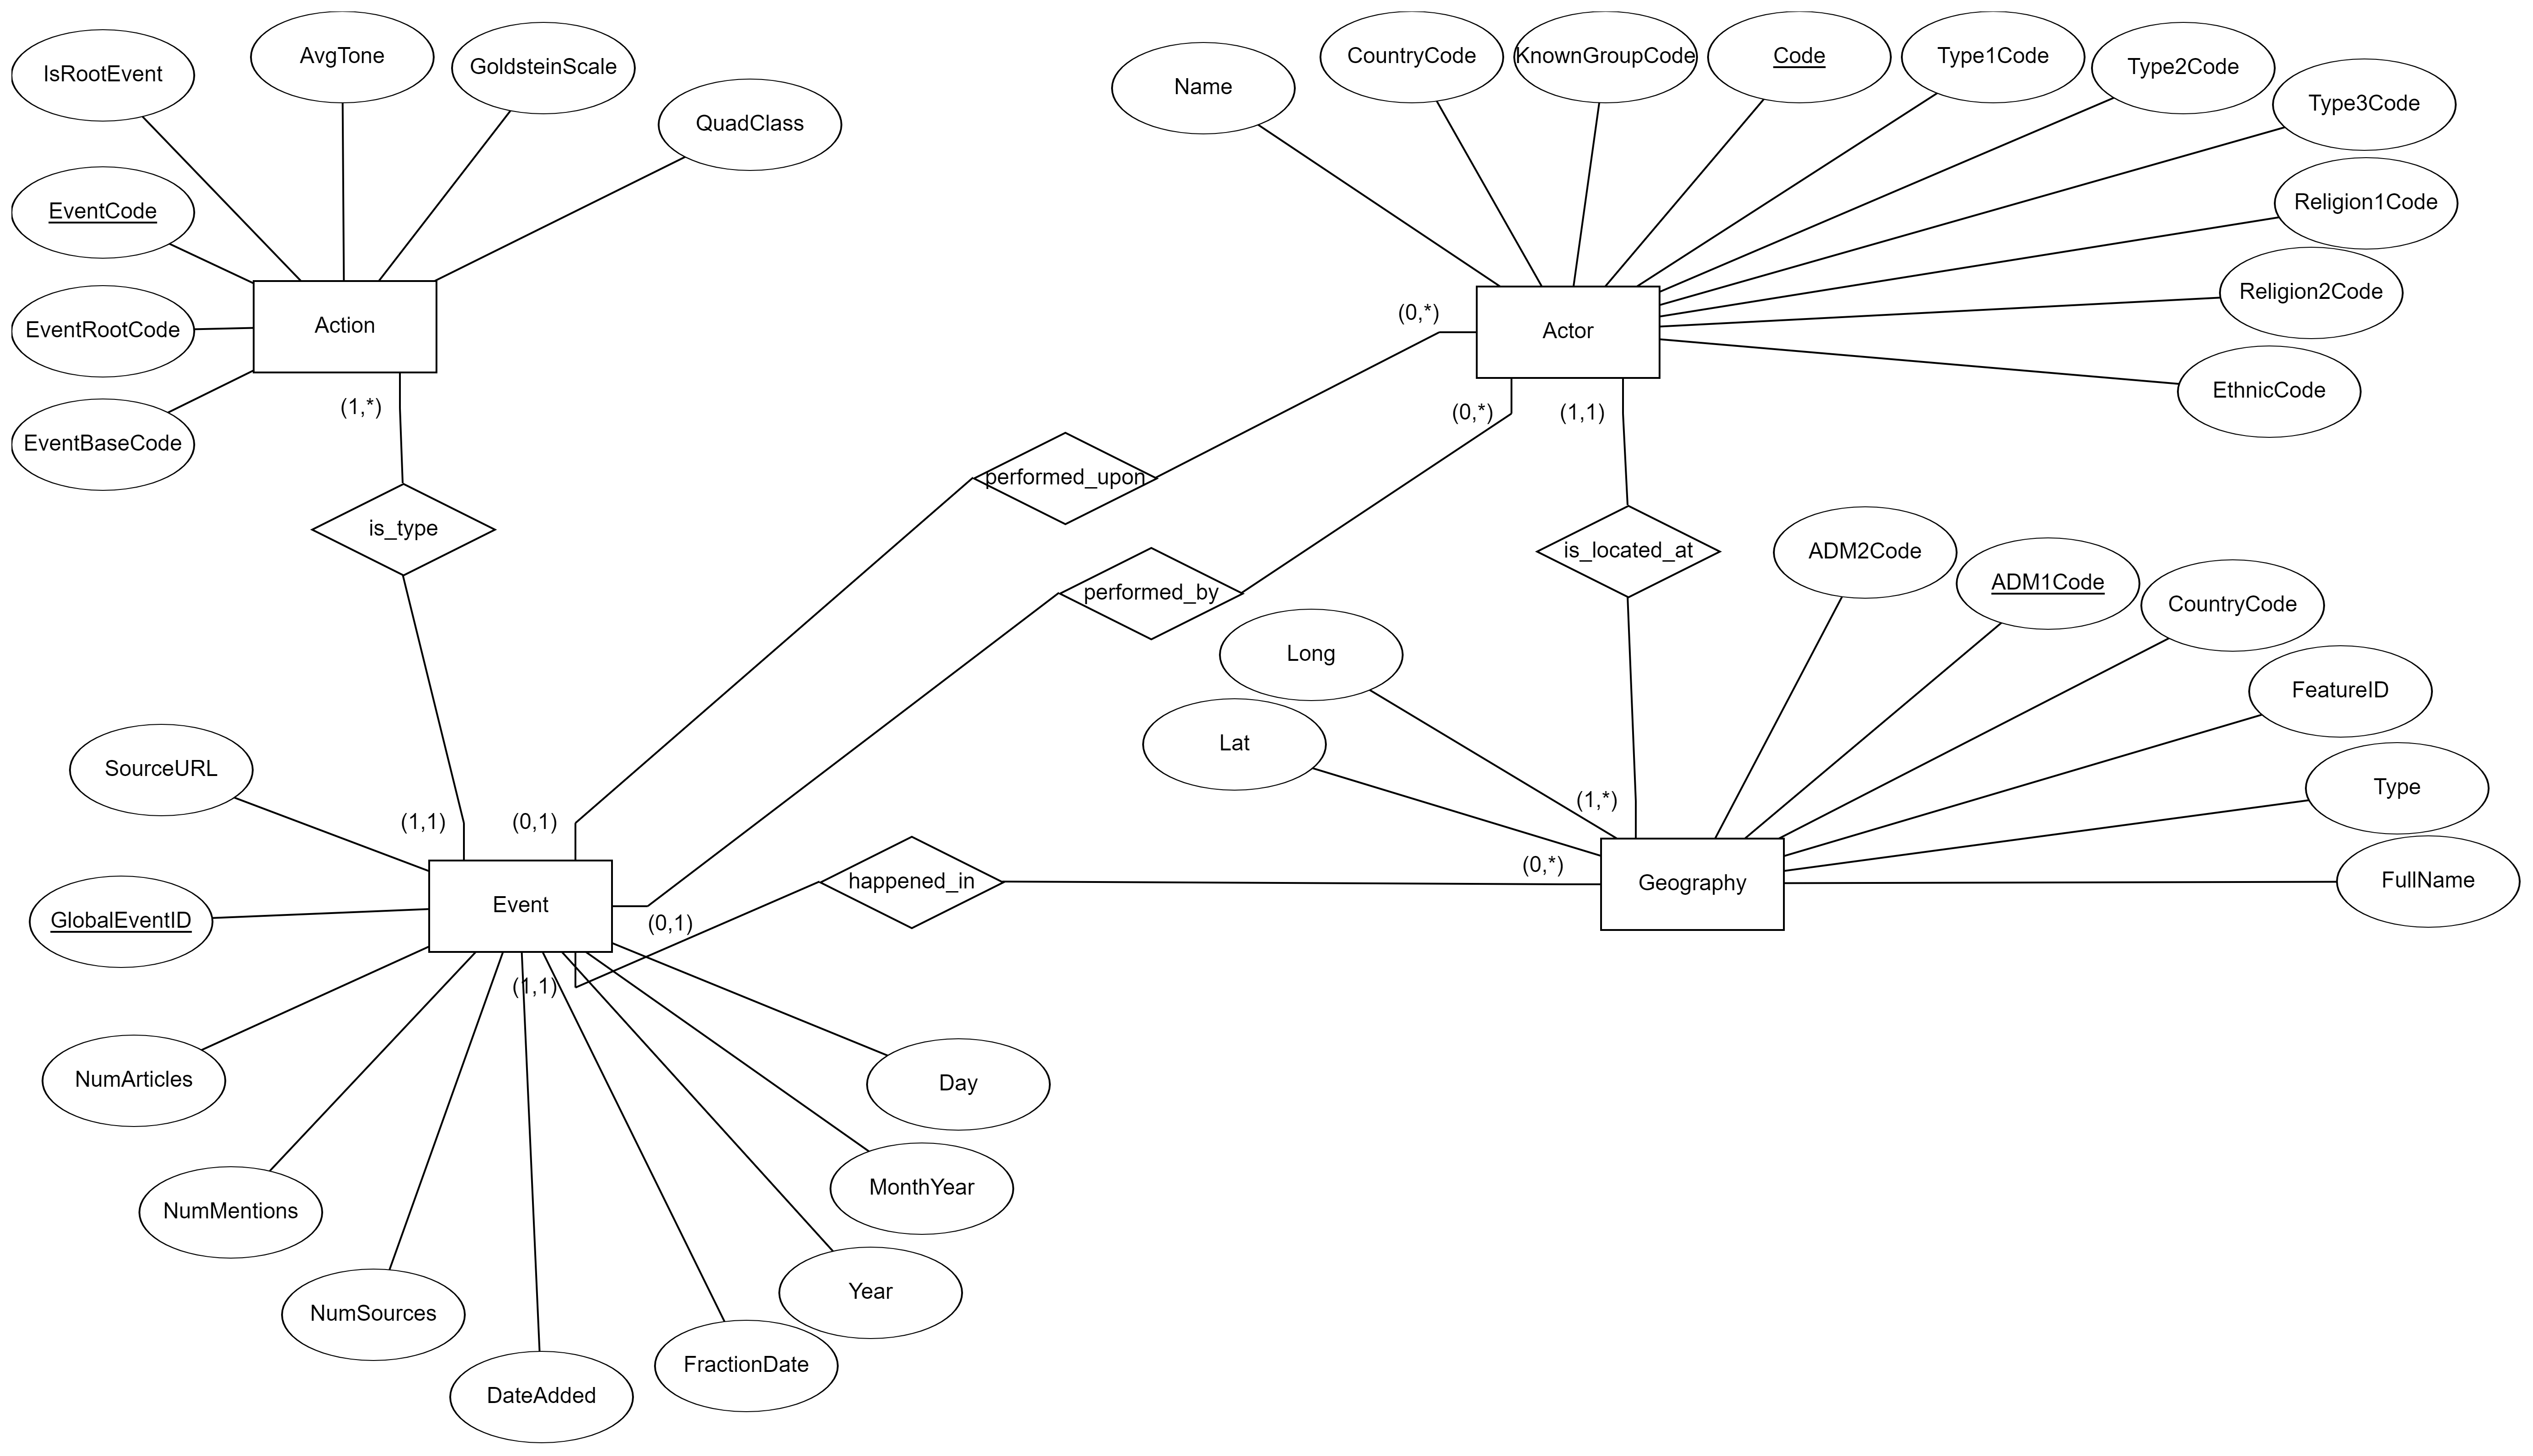
\includegraphics[scale = 0.08]{g9-gdelt}
	\caption{Our GDELT schema integration}
	\label{fig:gdelt}
\end{figure}

\begin{figure}
	\centering
	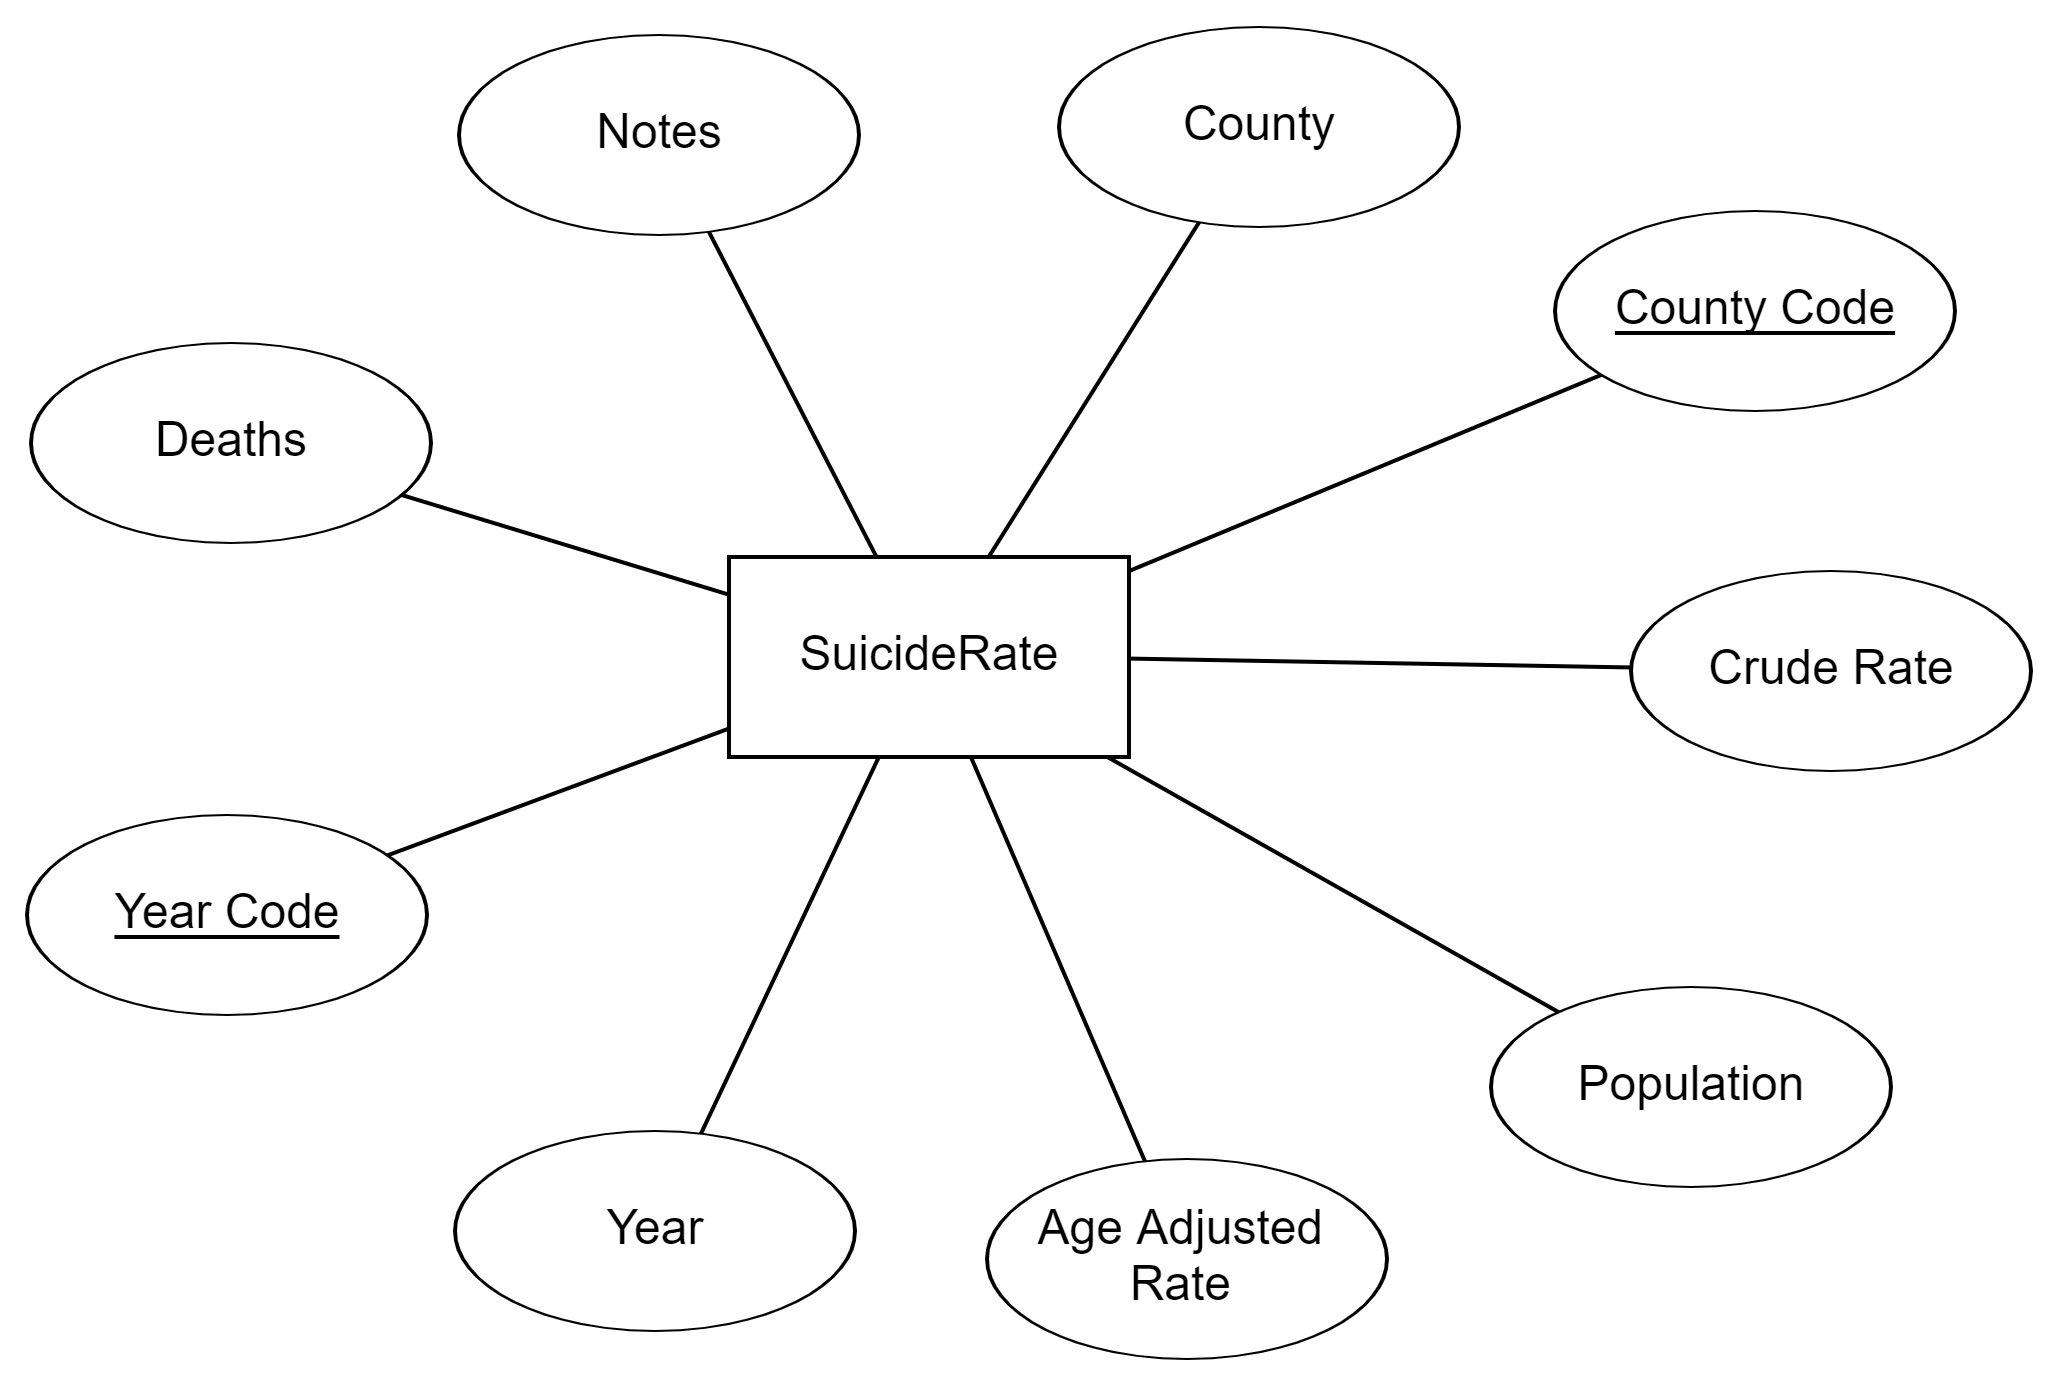
\includegraphics[scale = 0.18]{g9-suicide_rate}
	\caption{Our suicide rate schema integration}
	\label{fig:suicide_rate}
\end{figure}

\begin{figure}
	\centering
	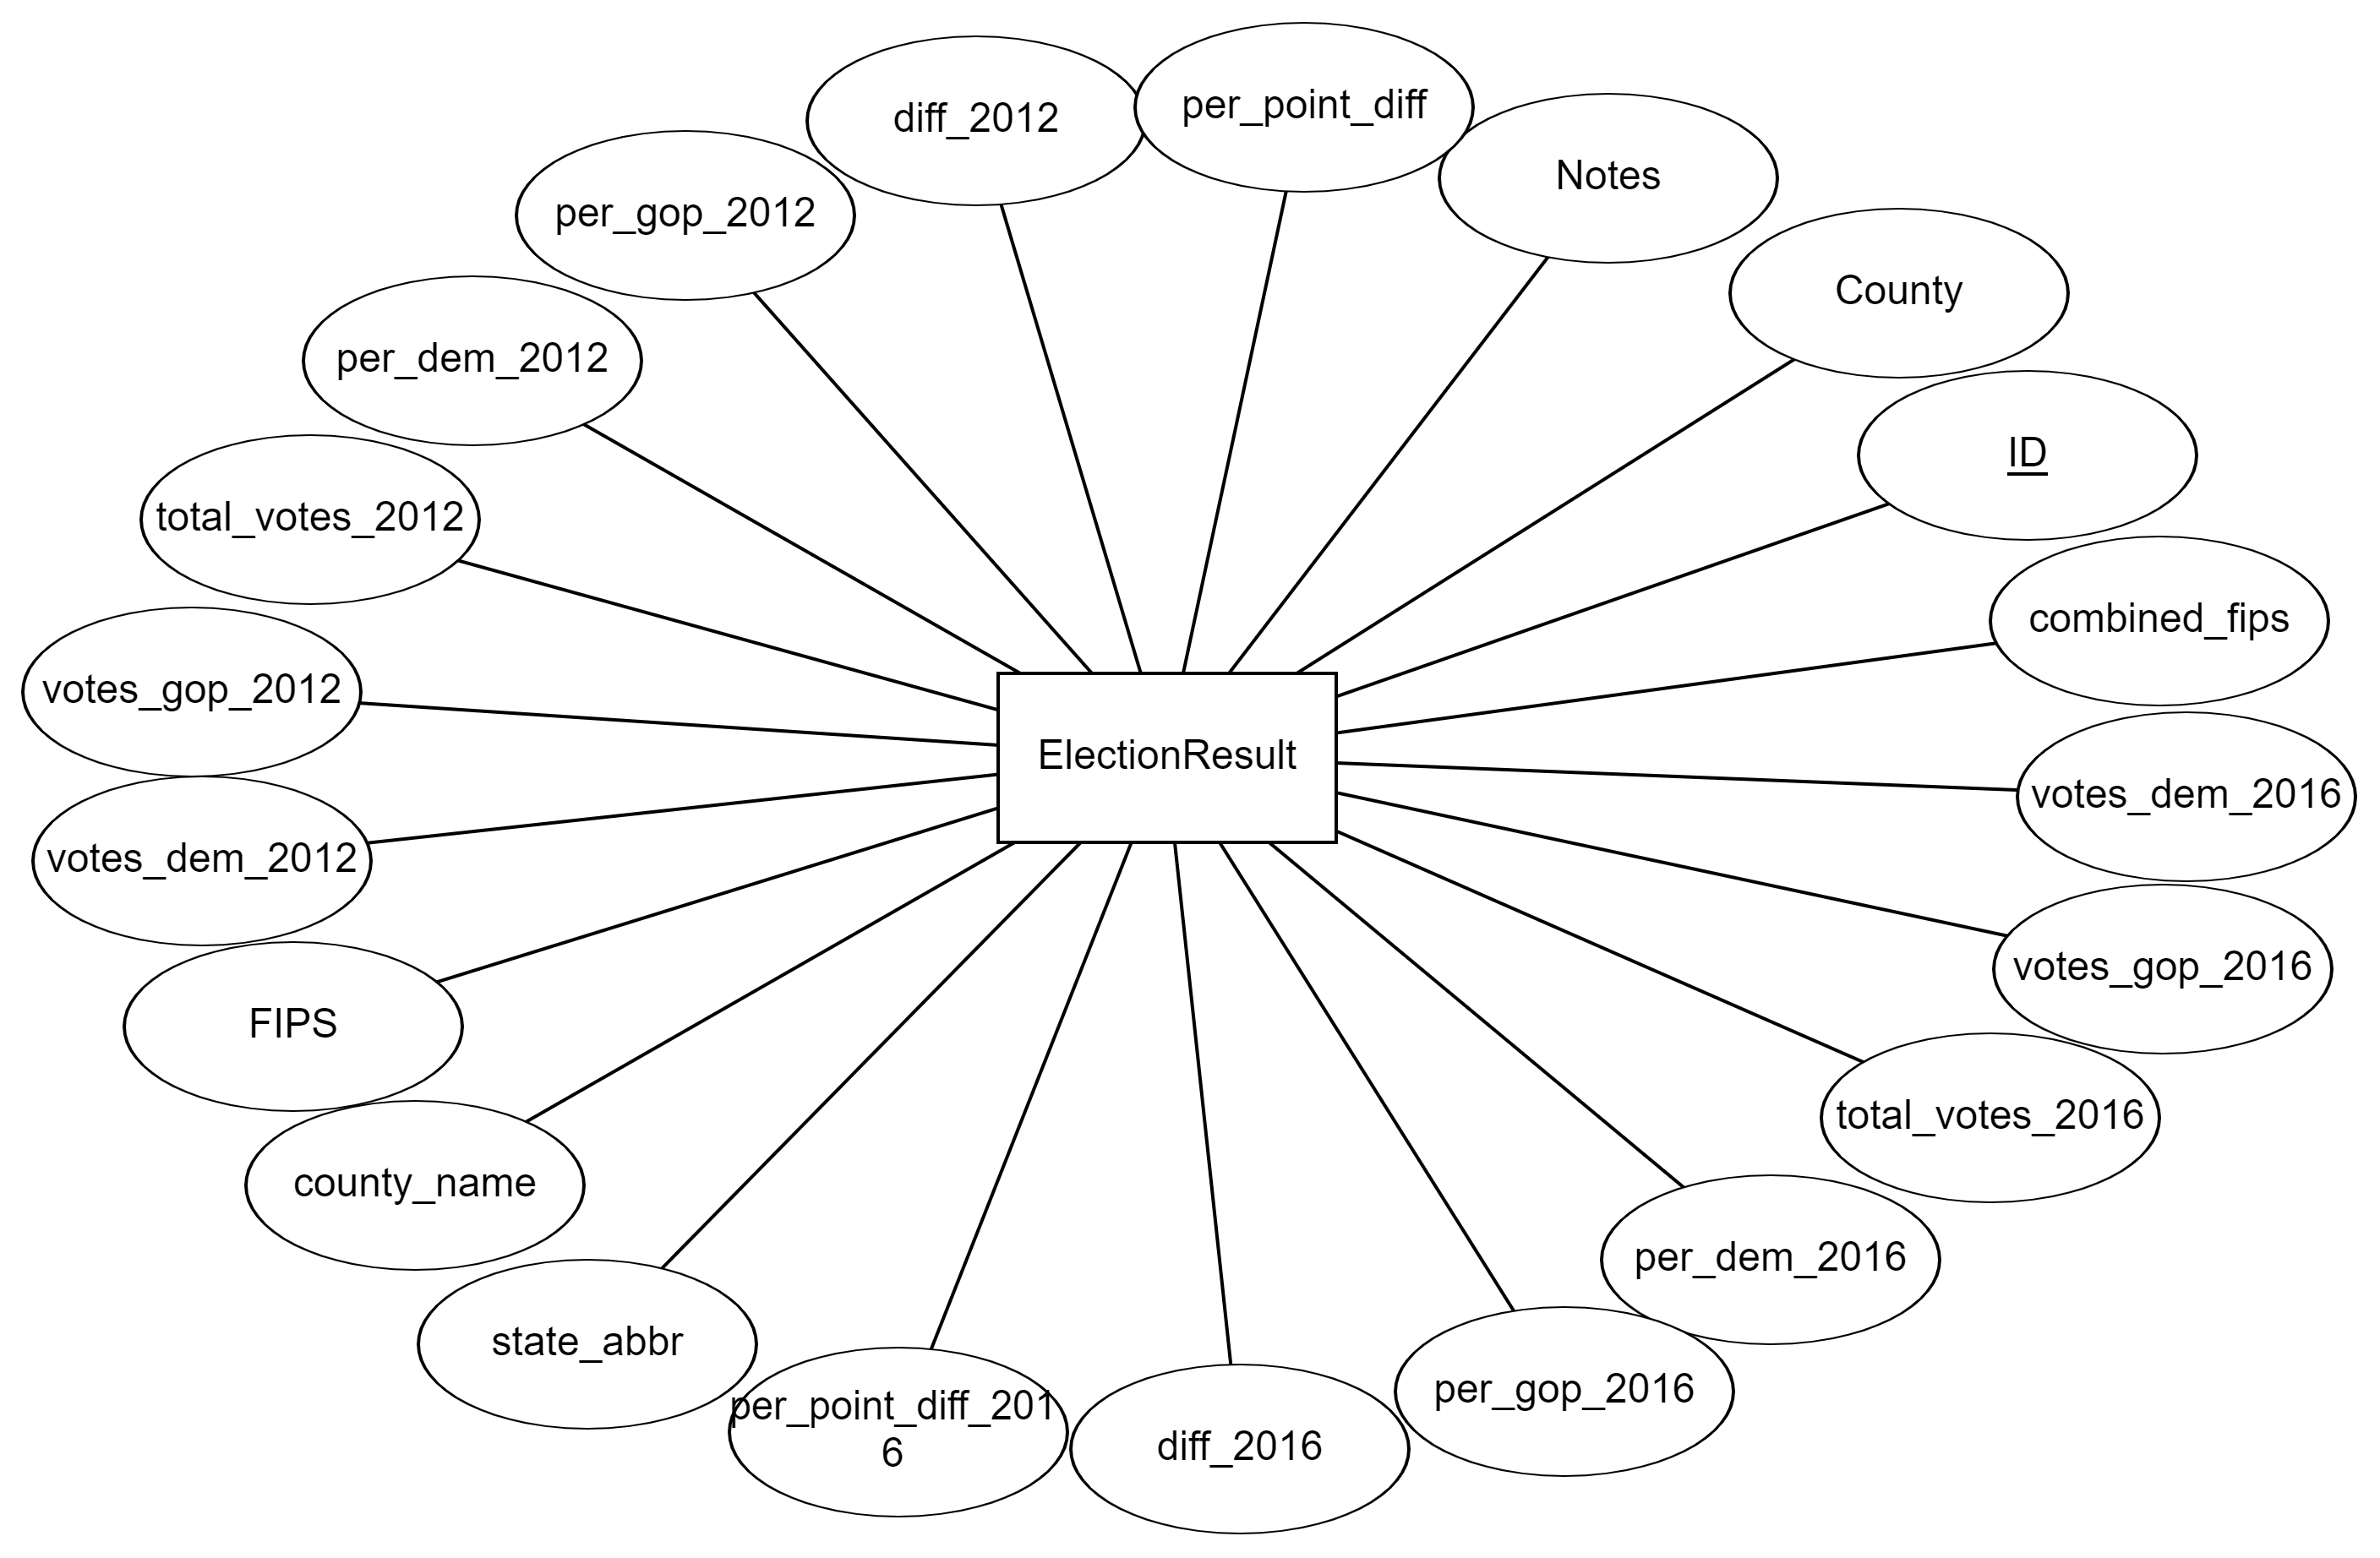
\includegraphics[scale = 0.12]{g9-election_results}
	\caption{Our election results integration}
	\label{fig:election_results}
\end{figure}

\begin{figure}
	\centering
	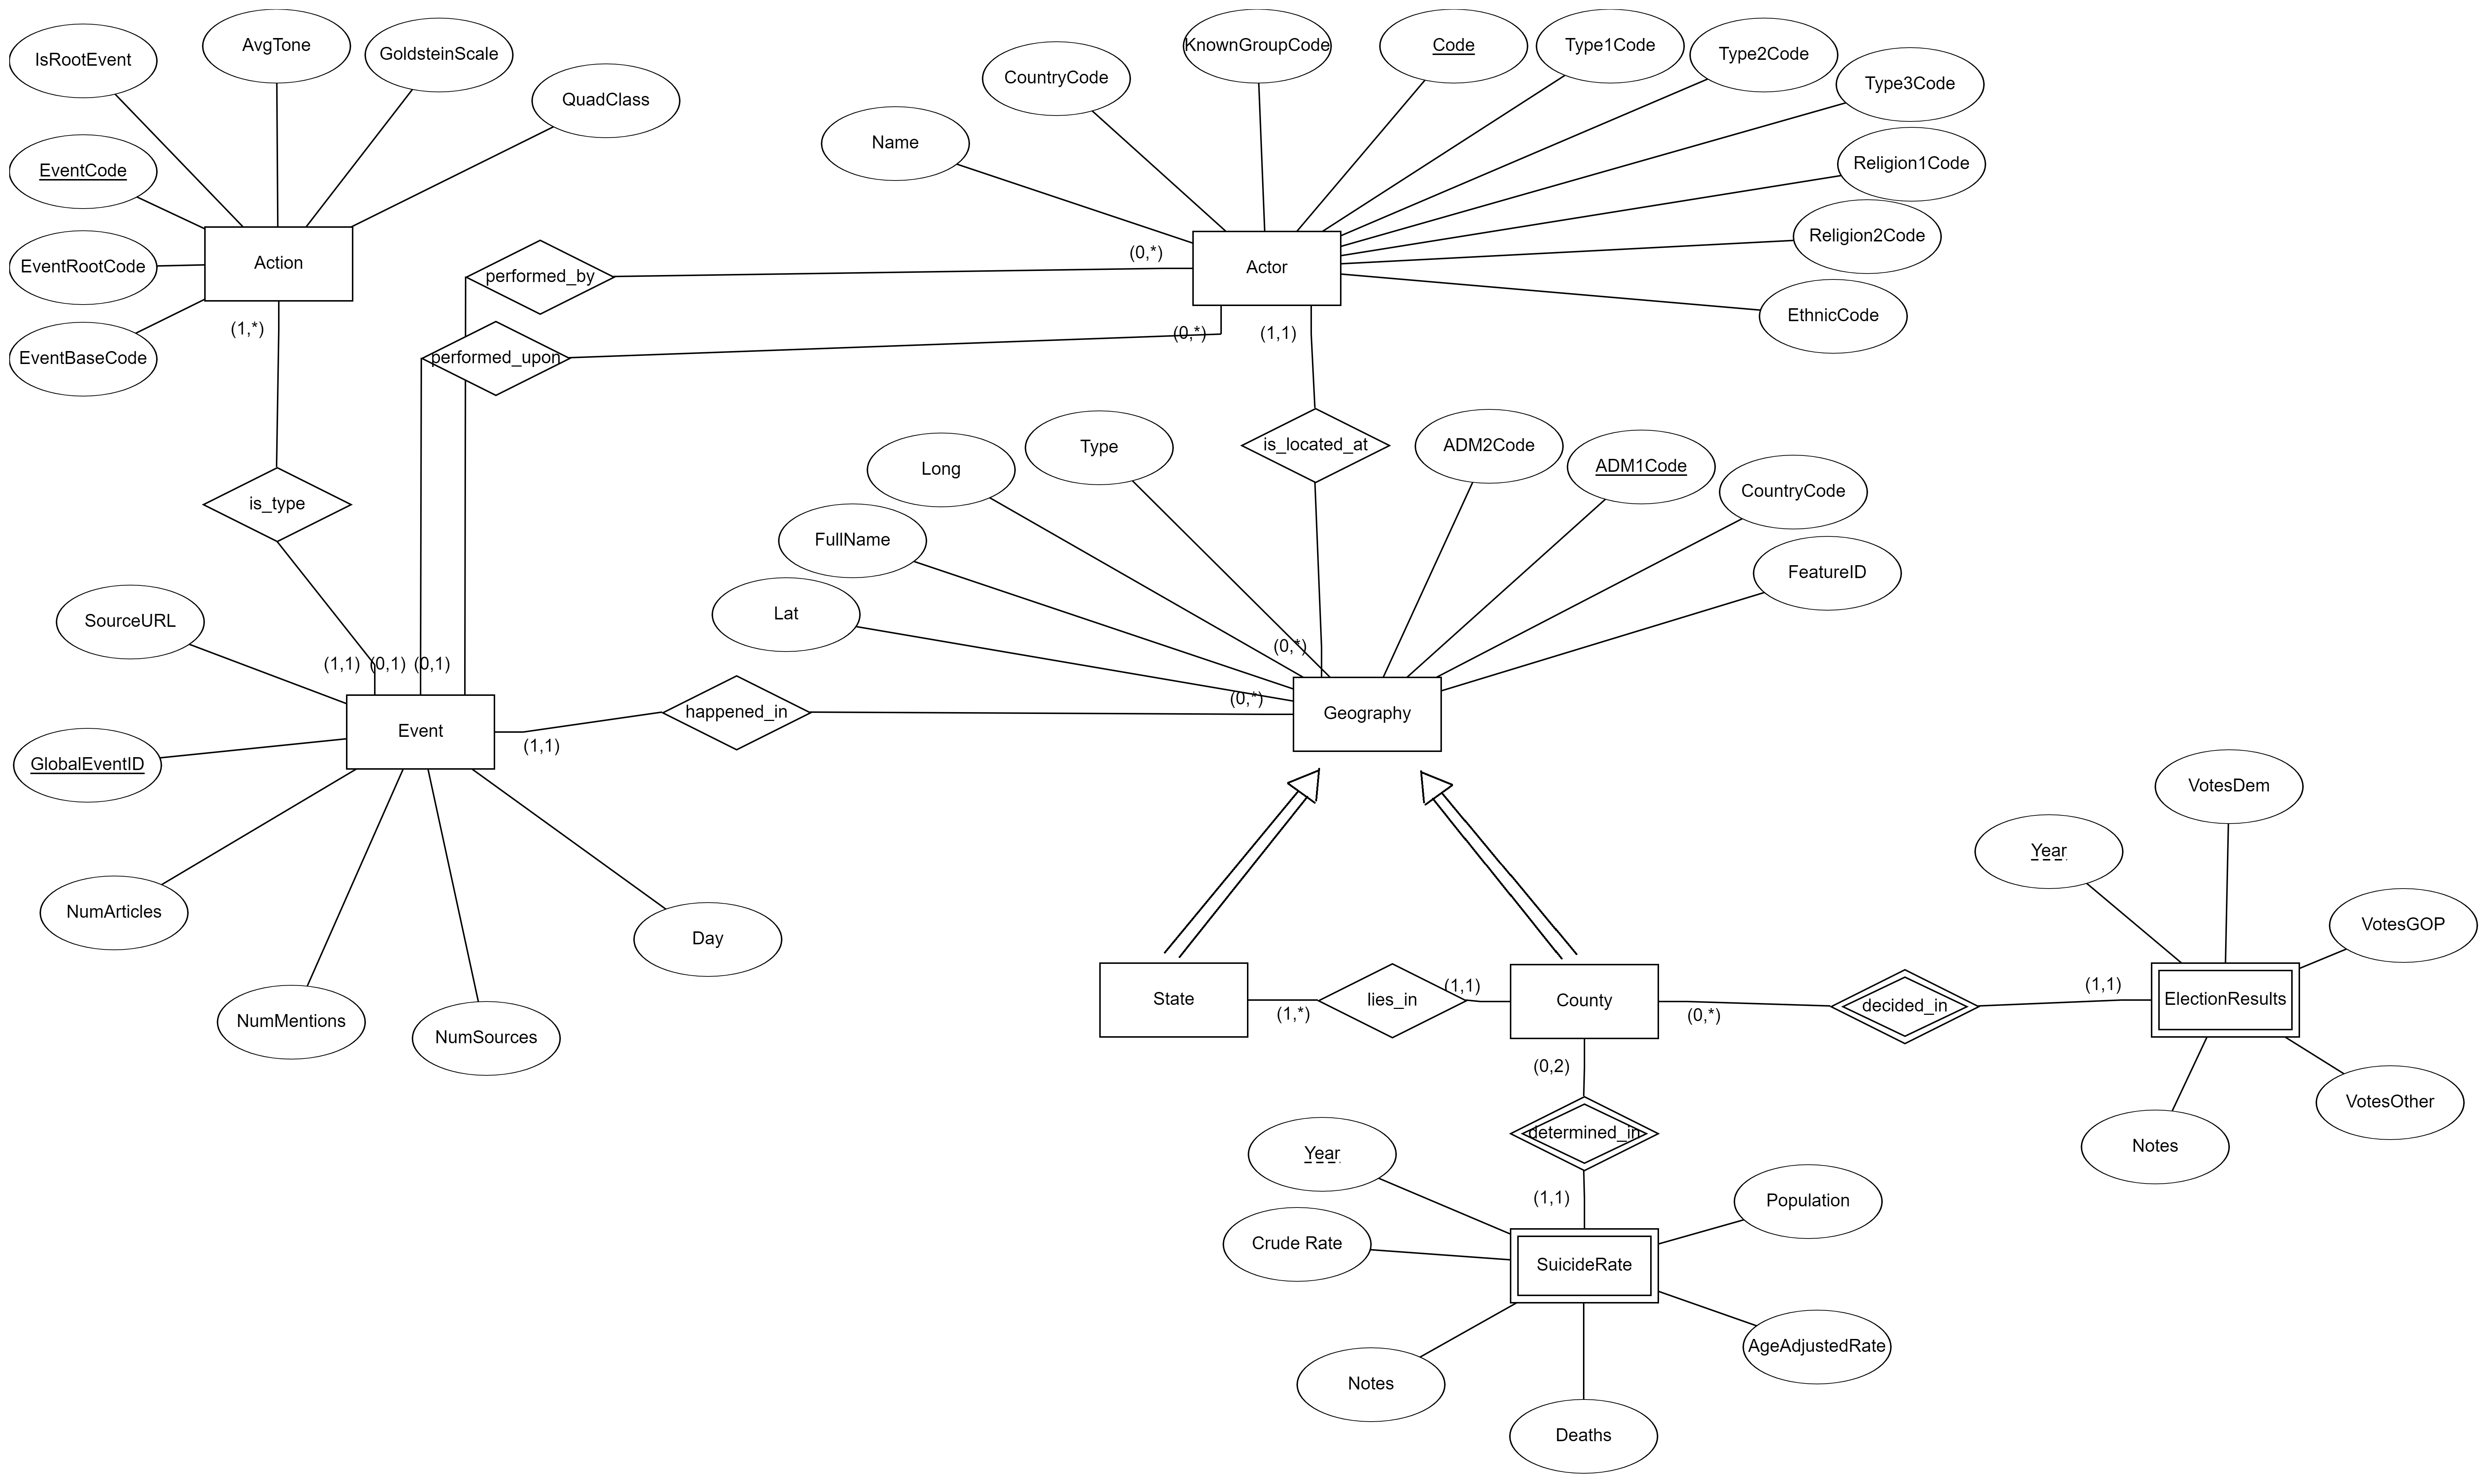
\includegraphics[scale = 0.08]{g9-all}
	\caption{Schema over the whole database}
	\label{fig:all}
\end{figure}


\textbf{Putting it all together}:
The election results and the Suicide Rate data sets have the
county attribute in common.
A county lies in a state, and both a county and a state are
spesializations of a "geography".
Some other attributes can be removed since they are redundant
(e.g. MonthYear makes the Year attribute irrelevant).
The end result can be seen on figure \ref{fig:all}.

\textbf{Technical parts}
On the inegration process, we tried using the counties' FIPS codes
present on each of the datasets to link the different entities
together.
However we quickly learned that each dataset's FIPS code
contradicts the FIPS code each other data set.

Our solution has been to identify each county (and state)
by a geoID code than can be derived from {\color{red}{todo
https://community.esri.com/thread/24614
ESRI
}}.

The only other hazard occurs when ElectionResults generates an
ID that does not match any County, in that case the corresponding
row is simply skipped and also printed to STDOUT for reference.


\section{DATA ANALYSIS}
The main and most important part.
We use sql queries to filter out the data that we need, make a bunch of plots and document everything.
We try to be as objective as possible.


\section{INTERPRETATION}
Why are the results the way they are?


\section{CONCLUSION}
final words



%\bibliographystyle{plain}
%\bibliography{biblist}

\end{document}

}{
    \import{reportContent/}{reportContent.tex}
}
\end{document}

% =======================================================================================
% =======================================================================================
% === IMPORTANT NOTE FOR STUDENTS:                                                    ===
% =======================================================================================
% === Do NOT change anything in this file. Only change files in the "reportContent"   ===
% === subfolder.                                                                      ===
% =======================================================================================
% =======================================================================================